%The paper size, font size and document type are defined in the following
\documentclass[a4paper,12pt]{article}

%Uncomment the following line, if you write in Finnish (special characters)
%\usepackage[utf8]{inputenc}

%\usepackage[finnish]{babel}
\usepackage[english]{babel}

%useful special symbols:
\usepackage{amssymb}
\usepackage{latexsym}
\usepackage{amsmath}
\usepackage{amsthm}

%a useful package if you write url addresses:
\usepackage{url}

%a package for figures:
\usepackage[dvips]{color}
\usepackage{epsfig}

%a package for rotated figures and tables:
\usepackage{rotating}




%if you want smaller page margins, uncomment and adjust the following
%\textheight=24.3cm
%\topmargin=-1.8cm
%\textwidth=16.7cm
%\oddsidemargin=-0.3cm
%\evensidemargin=0.0cm


%Create your own environments
\newtheorem{definition}{Definition}
\newtheorem{example}{Example}
\newtheorem{theorem}{Theorem}

%and useful macrosfor faster writing (benefit: you can change the notations 
%later, e.g., two possible notations for your vector x)
\newcommand{\Mmatr}{\ensuremath{\mathbf{M}}}
\newcommand{\xvec}{\ensuremath{\overline{x}}}
\newcommand{\xvecII}{\ensuremath{\mathbf{x}}} %alternative def
\newcommand{\Xset}{\ensuremath{\mathbf{X}}}
\newcommand{\fr}{\ensuremath{\mathit{fr}}} %just neater typing

%If you want to remove the space before paragraphs uncomment the following.
%Remember then to leave an empty line between paragraphs! 
%\setlength{\parindent}{0pt}


\title{MDM-2024 Homework N}
\author{Cuong Nguyen (101559968), Petteri Raita (ID2), and Raihan Gafur (ID3)}

%Uncomment the following, if you don't want the date to be printed
%\date{}

\begin{document}

\maketitle

\section{General instructions}

In the beginning, tell always the course name, homework number and
the authors' names and student identifiers. You can use a separate cover
page for these if you like.

The report structure (sections) is described in the task.  Typically,
the first section is ``Methods'', where you should describe briefly
how you solved the task. Mention here if you used some tool or made a
script (given in the appendix) and give references if you used any
external sources (i.e., other than the textbook and other course
material).

The results are usually presented in several sections. In addition to
text, there may be tables or figures.  Remember to give table row and
column labels and add required lables to plots (e.g., axis names in
scatter-plots) so that they are comprehensible. Mention important
observations in tables or figures in the text. Please try to make a
good layout. A table or figure in the middle of the page surrounded by
blank is not reader-friendly. Often, you are asked to interprete or
discuss the results. Try to explain {\em why} the things happen
instead of only decribing what has happened.

The last section is usually Appendix, where you should include the
code you used to produce your results. (In some tasks, there may be
multiple appendices.) If you used multiple external sources, give the
list of references in the end under caption``References''. (One
reference can be included in ``Methods'' as well.)


Remember all good habits that make presentation easily readable to
another person (e.g., rounding numbers to suitable precision,
introducing your own abbreviations). When using library functions
(e.g., for goodness measures), remember to check that the function
really calculates what is asked (the name of the function does not
guarantee this). If there are alterative ways to do something, tell
which one you chose (e.g., did you use biased or corrected estimates
of standard deviation), because they can lead to different results.

\section{Examples of tables and figures}

Table \ref{tab1a} and Figure \ref{figLDplot} show examples of including tables and figures.

\begin{table}[!h]
  \begin{center}
    \caption{Comparison of three clustering methods for $K=9$. SI=Silhouette index, CH=Calinski-Harabasz index, DB=Davies-Bouldin index.}
    \label{tab1a}
    \begin{tabular}{|l|r|r|r|}
      \hline
      method       & SI    & CH    & DB    \\
      \hline
      $K$-means    & 0.541 & 182.0 & 0.692 \\
      single-link  & 0.389 & 48.9  & 0.510 \\
      complete-lin & 0.469 & 129.5 & 0.731 \\
      \hline
    \end{tabular}
  \end{center}
\end{table}


\begin{figure}[!h]
  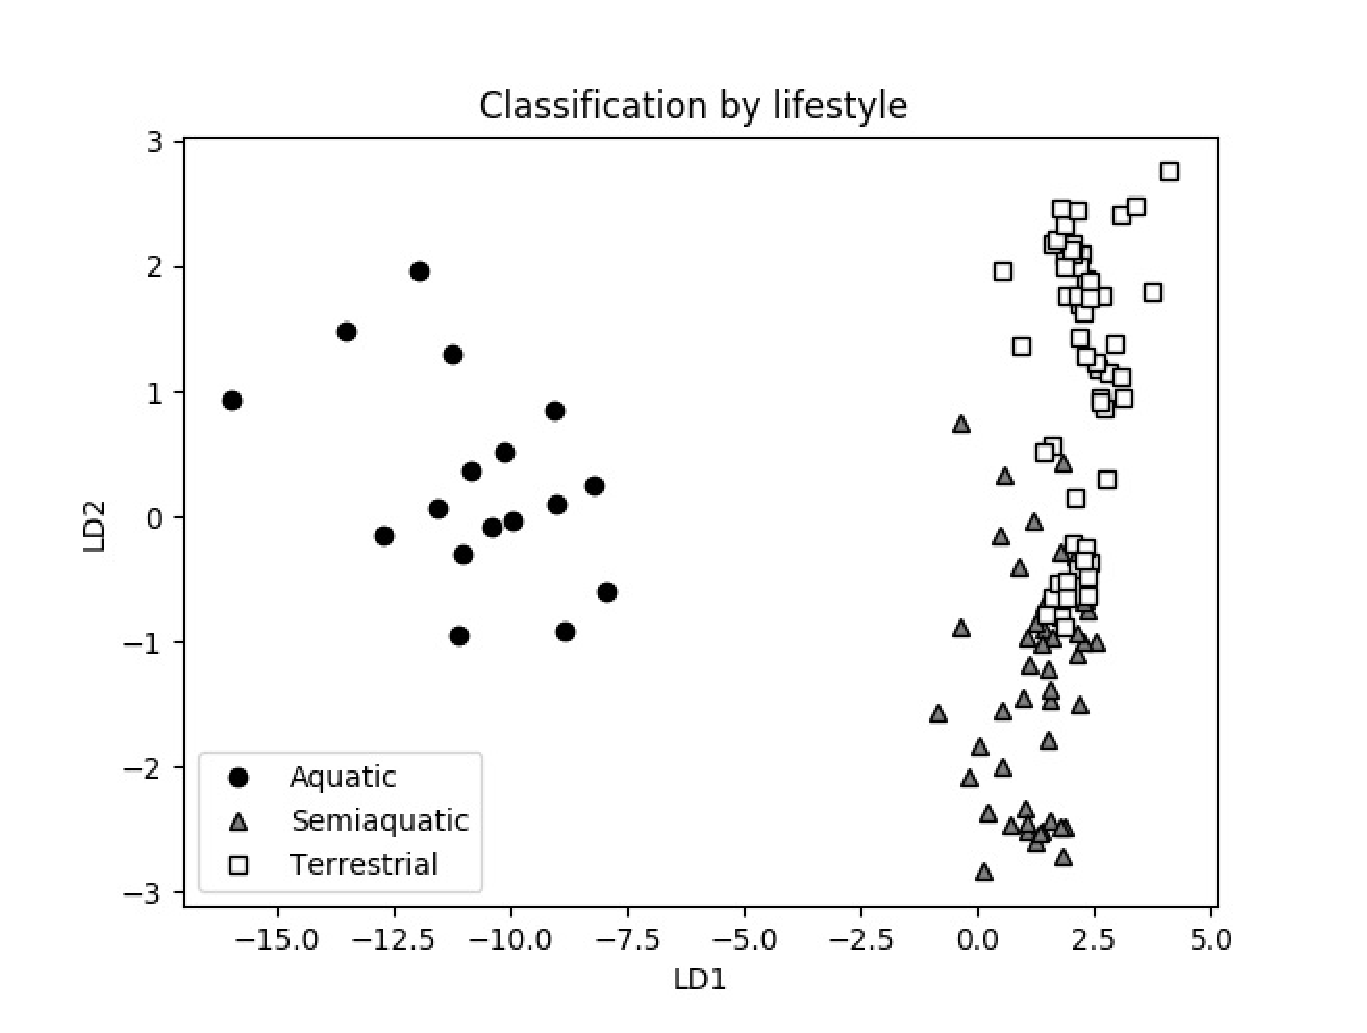
\includegraphics[width=\textwidth]{exLDplot.eps}
  \caption{Scatter plot of the data points and their classes along the first linar discriminants (LD1 and LD2).}
  \label{figLDplot}
\end{figure}


\section{Examples of references}

Here is an example of refering to
the original papers where Silhouette \cite{SI} and Calinski-Harabasz \cite{CH} indices were introduced.
Use references also to give credit to your sources. E.g., if you
wanted to explain the intuition of Calinski-Harabasz index
and found useful information in CrossValidated and wikipedia, you can
write like this

``Glen\_b in CrossVlidated \cite{glennCV} gave a useful hint that CH
is actually analogous to the $F$-ratio in ANOVA...'' ``According to Wikipedia \cite{Fwiki}, the ANOVA $F$-test statistic is...


\section{Some math examples and macros}

Typing math is probably the funniest thing with latex! Furthermore,
you can define new commands for notations you need often. In the
prememable, we have given new commands for $\Mmatr$

$$\Mmatr=\left[
    \begin{array}{ccc}
      a & b & c \\
      d & e & f \\
      g & h & i \\
    \end{array}\right]$$

and two alternative definitions for the vector, $\xvec$ and $\xvecII$ (to choose from).

Here is one example equation (cumulative hypergeometric probability):

$$p_F=\sum_{i=0}^J\frac{\left(\fr(\Xset) \atop \fr(\Xset C)+i
    \right) \left(\fr(\neg \Xset) \atop \fr(\neg \Xset \neg C)+i \right)}{\left(
    n
    \atop \fr(C)\right)},$$

where $J=\min\{\fr(\Xset\neg C),\fr(\neg X,C)\}$.

%Bibliography style. The alpha style generates references with 
%first letters and year. If you prefer numbers, use style plain.
% \bibliographystyle{alpha}
\bibliographystyle{plain}
%If you use bibtex, uncomment the following line and add your bibtex collection file (here ref.bib)
%\bibliography{ref} 

%another alternative is to type the list of references like here:
\begin{thebibliography}{1}

  \bibitem{CH}
  T.~Caliński and J.~Harabasz. A dendrite method for cluster analysis.
    {\em Communications in Statistics}, 3(1):1--27, 1974.


  \bibitem{glennCV}
  Glen\_b. Intuition behind the calinski-harabasz index. Answer in CrossValidated 2014.
  \url{https://stats.stackexchange.com/questions/97429/intuition-behind-the-calinski-harabasz-index}, accessed 10th Sep 2024.

  \bibitem{SI}
  Peter~J. Rousseeuw. Silhouettes: A graphical aid to the interpretation and validation of cluster analysis. {\em Journal of Computational and Applied Mathematics}, 20:53--65, 1987.

  \bibitem{Fwiki}
  Wikipedia contributors. F-test, 2024.
  \url{https://en.wikipedia.org/wiki/F-test}, Accessed 29th Aug 2024.

\end{thebibliography}

\end{document}
